% --------------------------------------------------------------
% This is all preamble stuff that you don't have to worry about.
% Head down to where it says "Start here"
% --------------------------------------------------------------
 
\documentclass[12pt]{article}

\usepackage[margin=1in]{geometry} 
\usepackage{amsmath,amsthm,amssymb}
\usepackage[margin=1in]{geometry} 
\usepackage{amsmath,amsthm,amssymb}
%\usepackage[spanish]{babel} %Castellanización
\usepackage[T1]{fontenc} %escribe lo del teclado
\usepackage{inputenc} %Reconoce algunos símbolos
\usepackage{lmodern} %optimiza algunas fuentes
\usepackage{graphicx}
\graphicspath{ {images/} }
\usepackage{hyperref} % Uso de links

% To Display Chinese words
\usepackage{xeCJK}
% To Display Code
% \usepackage{listings}
\usepackage{minted}
% To Display csv file
\usepackage{csvsimple}
\usepackage{longtable}
\usepackage{booktabs}
 
\newcommand{\N}{\mathbb{N}}
\newcommand{\Z}{\mathbb{Z}}
 
\newenvironment{theorem}[2][Theorem]{\begin{trivlist}
\item[\hskip \labelsep {\bfseries #1}\hskip \labelsep {\bfseries #2.}]}{\end{trivlist}}
\newenvironment{lemma}[2][Lemma]{\begin{trivlist}
\item[\hskip \labelsep {\bfseries #1}\hskip \labelsep {\bfseries #2.}]}{\end{trivlist}}
\newenvironment{exercise}[2][Exercise]{\begin{trivlist}
\item[\hskip \labelsep {\bfseries #1}\hskip \labelsep {\bfseries #2.}]}{\end{trivlist}}
\newenvironment{problem}[2][Problem]{\begin{trivlist}
\item[\hskip \labelsep {\bfseries #1}\hskip \labelsep {\bfseries #2.}]}{\end{trivlist}}
\newenvironment{question}[2][Question]{\begin{trivlist}
\item[\hskip \labelsep {\bfseries #1}\hskip \labelsep {\bfseries #2.}]}{\end{trivlist}}
\newenvironment{corollary}[2][Corollary]{\begin{trivlist}
\item[\hskip \labelsep {\bfseries #1}\hskip \labelsep {\bfseries #2.}]}{\end{trivlist}}

\newenvironment{solution}{\begin{proof}[Solution]}{\end{proof}}

% write csv content in latex 
\begin{filecontents*}{grade.csv}
name,givenname,matriculation,gender,grade
Maier,Hans,12345,m,1.0
Huber,Anna,23456,f,2.3
Weisbaeck,Werner,34567,m,5.0
\end{filecontents*}
 
\begin{document}
 
% --------------------------------------------------------------
%                         Start here
% --------------------------------------------------------------
 
\title{2019 Deep Learning and Practice \\ Lab 5 \\ Conditional Sequence-to-sequence VAE}
\author{0756110 李東霖}

\maketitle
\section{Introduction}

Every English verb has its tenses like simple、simple past etc. To convert different tense between input words and target words, this lab use tense as condition and English words as input and target.

Some requirements as follows:

\begin{itemize}
\item Implement a C seq2seq VAE model.
\item Adopt two method which teacher-forcing and kl loss annealing to train model.
\item Plot cross-entropy loss and kl loss curves during training.
\item Plot the BLEU-4 score curve of the test data during training
\item Show the results generated words with 4 tenses by Gaussian normal distribution.
\end{itemize}

\section{Implementation details}

\subsection{Dataloader}

To feed character into model, I converted character to number by \verb|Dictionary|. But I direct added 26 English character and 2 special token (<SOS> and <EOS>) into \verb|Dictionary|. After that I implemented some convenient function to convert string between \verb|LongTensor| one-hot.

\begin{minted}[frame=lines]{python}
class CharDict:
    def __init__(self):
        self.word2index = {}
        self.index2word = {}
        self.n_words = 0
        
        for i in range(26):
            self.addWord(chr(ord('a') + i))
        
        tokens = ["SOS", "EOS"]
        for t in tokens:
            self.addWord(t)

    def addWord(self, word):
        if word not in self.word2index:
            self.word2index[word] = self.n_words
            self.index2word[self.n_words] = word
            self.n_words += 1

    def longtensorFromString(self, s):
        s = ["SOS"] + list(s) + ["EOS"]
        return torch.LongTensor([self.word2index[ch] for ch in s])
    
    def stringFromLongtensor(self, l, show_token=False, check_end=True):
        s = ""
        for i in l:
            ch = self.index2word[i.item()]
            if len(ch) > 1:
                if show_token:
                    __ch = "<{}>".format(ch)
                else:
                    __ch = ""
            else:
                __ch = ch
            s += __ch
            if check_end and ch == "EOS":
                break
        return s
\end{minted}

Then I created \verb|wordDataset| to load \verb|train.txt| and \verb|text.txt| dataset. Because the train and test data are very different format. I did some preprocessing with them. Finally, shapes of train and test data are $(\#data, 1)$ with string type. In \verb|__getitem__|, I return one word (\verb|LongTensor|) and tenses condition when training. And return two word (\verb|LongTensor|) with two tenses condition when testing.

\begin{minted}[frame=lines]{python}
class wordsDataset(Dataset):
    def __init__(self, train=True):
        if train:
            f = './train.txt'
        else:
            f = './test.txt'
        self.datas = np.loadtxt(f, dtype=np.str)
        
        if train:
            self.datas = self.datas.reshape(-1)
        else:
            self.targets = np.array([
                [0, 3],
                [0, 2],
                [0, 1],
                [0, 1],
                [3, 1],
                [0, 2],
                [3, 0],
                [2, 0],
                [2, 3],
                [2, 1],
            ])
        
        #self.tenses = ['sp', 'tp', 'pg', 'p']
        self.tenses = [
            'simple-present', 
            'third-person', 
            'present-progressive', 
            'simple-past'
        ]
        self.chardict = CharDict()
        
        self.train = train
    
    def __len__(self):
        return len(self.datas)
    
    def __getitem__(self, index):
        if self.train:
            c = index % len(self.tenses)
            return self.chardict.longtensorFromString(self.datas[index]), c
        else:
            i = self.chardict.longtensorFromString(self.datas[index, 0])
            ci = self.targets[index, 0]
            o = self.chardict.longtensorFromString(self.datas[index, 1])
            co = self.targets[index, 1]
            
            return i, ci, o, co
\end{minted}

\subsection{Encoder}

In seq2seq, data $x$ before start token are inputs and data $y$ after start token are targets. So separate seq2seq at there as encoder and decoder. In CVAE, encoder generates latent vector $z$ by fed $x$ and decoder generate target output $y$ by fed $z$. 
\par \ \par
In the begin, I convert condition one-hot to embedding vector and concatenate it with initial hidden input. After that I also convert inputs one-hot to embedding vector (use different embedding layer between condition). To avoid too many hidden parameters, I chose \verb|nn.GRU| as my RNN implementation. And I fed all inputs data and initial hidden with condition into RNN to get last hidden output. Now, I need to generate latent vector $z$.

\subsubsection{Variational latent vector}

In VAE, the latent vector distribution are multivariate Gaussian distribution. Therefore I need to get mean and variance from hidden output through \verb|nn.Linear| layers. Here has one problem on variance. In definition, variance is always positive. But linear output possible be negative. To solve that problem, redefine linear output is log variance. From to now, I get multivariate Gaussian distribution from encoder. Here has another problem appeared. Let us see next subsection.

\subsubsection{Reparameterization trick}

A new problem isHere hings another problem appeared. distribution can't calculate gradient for parameters of encoder. That means I can't train encoder by decoder output loss. Reparameterization trick is solution for this problem. First, sample a $z^*$ from multivariate normal distribution $\sim N(0,1)$ . Second, use equation \ref{trick} to get $z$.

\begin{equation}
\label{trick}
z = z^* * \exp(logvar/2) + mean
\end{equation} 

Finally, I get $z$ from $N(mean, \exp(logvar))$. In compute graph perspective, it only multiple a constant for mean and log variance. Therefore it also can calculate gradient for parameters of encoder.

\begin{minted}[frame=lines]{python}
class EncoderRNN(nn.Module):
    def __init__(
        self, word_size, hidden_size, latent_size, 
        num_condition, condition_size
    ):
        super(EncoderRNN, self).__init__()
        self.word_size = word_size
        self.hidden_size = hidden_size
        self.condition_size = condition_size
        self.latent_size = latent_size

        self.condition_embedding = nn.Embedding(num_condition, condition_size)
        self.word_embedding = nn.Embedding(word_size, hidden_size)
        self.gru = nn.GRU(hidden_size, hidden_size)
        self.mean = nn.Linear(hidden_size, latent_size)
        self.logvar = nn.Linear(hidden_size, latent_size)

    def forward(self, inputs, init_hidden, input_condition):
        c = self.condition(input_condition)
        
        # get (1,1,hidden_size)
        hidden = torch.cat((init_hidden, c), dim=2)
        
        # get (seq, 1, hidden_size)
        x = self.word_embedding(inputs).view(-1, 1, self.hidden_size)
        
        # get (seq, 1, hidden_size), (1, 1, hidden_size)
        outputs, hidden = self.gru(x, hidden)
        
        # get (1, 1, hidden_size)
        m = self.mean(hidden)
        logvar = self.logvar(hidden)
        
        z = self.sample_z() * torch.exp(logvar/2) + m
        
        return z, m, logvar

    def initHidden(self):
        return torch.zeros(
            1, 1, self.hidden_size - self.condition_size, 
            device=device
        )
    
    def condition(self, c):
        c = torch.LongTensor([c]).to(device)
        return self.condition_embedding(c).view(1,1,-1)
    
    def sample_z(self):
        return torch.normal(
            torch.FloatTensor([0]*self.latent_size), 
            torch.FloatTensor([1]*self.latent_size)
        ).to(device)
\end{minted}

\subsection{Decoder}

The seq2seq after start token is decoder, decoder need previous output to decide what current outputs. It just like we don't put verb after adjective. And also decoder can output end token to stop. In CVAE, decoder decode latent vector $z$ and condition $c$ then get output.

First, I convert latent vector $z$ and condition $c$ to hidden size through \verb|nn.Linear|. Second, I input $x$ through embedded layer in one time. It isn't like encoder can input all $x$ and get back all outputs. Because I also need to change $x$ between ground truth $y$ or model output $\hat{y}$. I will talk that in next sub section.

\begin{minted}[frame=lines]{python}
class DecoderRNN(nn.Module):
    def __init__(
        self, word_size, hidden_size, latent_size, condition_size
    ):
        super(DecoderRNN, self).__init__()
        self.hidden_size = hidden_size
        self.word_size = word_size

        self.latent_to_hidden = nn.Linear(
            latent_size+condition_size, hidden_size
        )
        self.word_embedding = nn.Embedding(word_size, hidden_size)
        self.gru = nn.GRU(hidden_size, hidden_size)
        self.out = nn.Linear(hidden_size, word_size)
    
    def initHidden(self, z, c):
        latent = torch.cat((z, c), dim=2)
        return self.latent_to_hidden(latent)
    
    def forward(self, x, hidden):
        # get (1, 1, hidden_size)
        x = self.word_embedding(x).view(1, 1, self.hidden_size)
        
        # get (1, 1, hidden_size) (1, 1, hidden_size)
        output, hidden = self.gru(x, hidden)
            
        # get (1, word_size)
        output = self.out(output).view(-1, self.word_size)
        
        return output, hidden
\end{minted}

\subsubsection{Teacher-forcing}

The decoder depend on previous output that causes one issue. If previous output is totally wrong, it will influence model and make training so hard. To solve issue, sometimes mandatory input ground truth into model can help quickly fit.

\begin{minted}[frame=lines]{python}
def decode_inference(decoder, z, c, maxlen, teacher=False, inputs=None):
    sos_token = train_dataset.chardict.word2index['SOS']
    eos_token = train_dataset.chardict.word2index['EOS']
    z = z.view(1,1,-1)
    i = 0
    
    outputs = []
    x = torch.LongTensor([sos_token]).to(device)
    hidden = decoder.initHidden(z, c)
    
    for i in range(maxlen):
        # get (1, word_size), (1,1,hidden_size)
        x = x.detach()
        output, hidden = decoder(
            x,
            hidden
        )
        outputs.append(output)
        output_onehot = torch.max(torch.softmax(output, dim=1), 1)[1]
        
        # meet EOS
        if output_onehot.item() == eos_token and not teacher:
            break
        
        if teacher:
            x = inputs[i+1:i+2]
        else:
            x = output_onehot
    
    # get (seq, word_size)
    if len(outputs) != 0:
        outputs = torch.cat(outputs, dim=0)
    else:
        outputs = torch.FloatTensor([]).view(0, word_size).to(device)
    
    return outputs
\end{minted}

\subsection{KL loss}

If the loss function only cares output accuracy, it can't prove the latent vector $z$ is Gaussian normal distribution $N(0, 1)$. So add KL loss as follows:

\begin{equation}
\begin{split}
& KL( N(u, \sigma^2) || N(0,1) ) \\ & = \int \frac{1}{\sqrt{2\pi \sigma^2}} e^{-\frac{(x-u)^2}{2\sigma^2}} \left( \log \frac{ e^{-\frac{(x-u)^2}{2\sigma^2}} / \sqrt{2\pi \sigma^2} }{ e^{\frac{-x^2}{2}} / \sqrt{2/pi} } \right) dx \\
& = \int \frac{1}{\sqrt{2\pi \sigma^2}} e^{-\frac{(x-u)^2}{2\sigma^2}} \log \left(  \frac{1}{\sqrt{\sigma^2}} \exp{\frac{1}{2} (x^2 - \frac{(x-u)^2}{\sigma^2}) } \right) dx \\
& = \int \frac{1}{\sqrt{2\pi \sigma^2}} e^{-\frac{(x-u)^2}{2\sigma^2}} \frac{1}{2} \left( -\log \sigma^2 + x^2 - \frac{(x-u)^2}{\sigma^2} \right) dx \\
& = \frac{1}{2} (-\log \sigma^2 + u^2 + \sigma^2 - 1)
\end{split}
\end{equation}

Implemented code as follows:

\begin{minted}[frame=lines]{python}
def KL_loss(m, logvar):
    return torch.sum(0.5 * (-logvar + (m**2) + torch.exp(logvar) - 1))
\end{minted}

And I need to trade off cross entropy and KLD each percent. Like this:

\begin{equation}
L = L_{CROSSENTROPY} + w * L_{KLD}
\end{equation}

\subsection{KL weight annealing}

I use epoch number to decide how much KLD weight.

\begin{minted}[frame=lines]{python}
def KLD_weight_annealing(epoch):
    slope = 0.001
    scope = (1.0 / slope)*2
    
    w = (epoch % scope) * slope
    
    if w > 1.0:
        w = 1.0
    
    return w
\end{minted}

\section{Experimental results}

To conveniently compare hyper parameters between loss and score, I combine all curves into one image.

\begin{figure}[H]
\centering
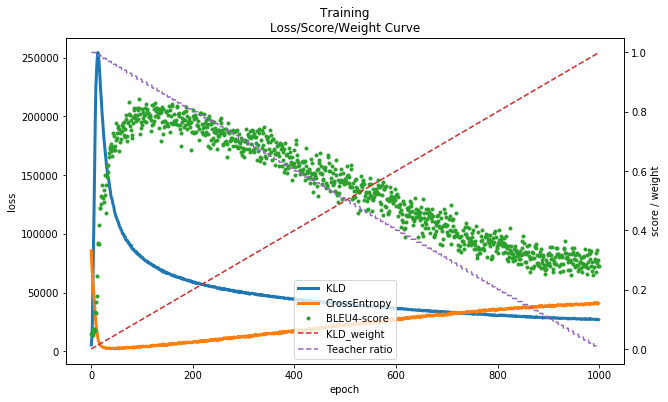
\includegraphics[width=\linewidth]{Images/curvesv2.png} 
\caption{Loss, Score, Weight Curves when training with lr=0.001}
\end{figure}

In the begin, the KLD weight is low then cause cross entropy loss became very lower and KLD loss became very higher. After higher KLD weight, the cross entropy became higher and KLD loss became lowwer. Because KLD weight changes objective function. I also find the high score corresponding low cross entropy loss. In order to generate words from decoder through Gaussian noise, I must decrease the KLD loss to make latent vector $z$ more closely with Gaussian normal distribution. But that makes lower score, this means I can't easy to encode all words into Gaussian normal distribution.

\section{Discussion}

\subsection{Teacher forcing ratio from 0 to 1}

\begin{figure}[H]
\centering
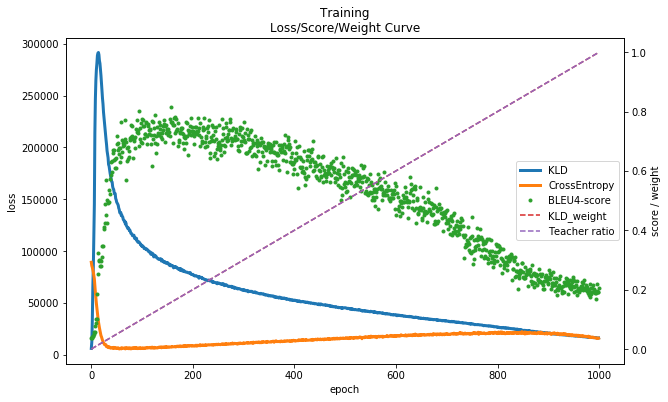
\includegraphics[width=\linewidth]{Images/curves.png} 
\caption{Loss, Score, Weight Curves when training with lr=0.001}
\end{figure}

I find the model also get good score when ratio=0 in begin.

\subsection{KL weight annealing}

I modify annealing curve to see its effects.

\begin{figure}[H]
\centering
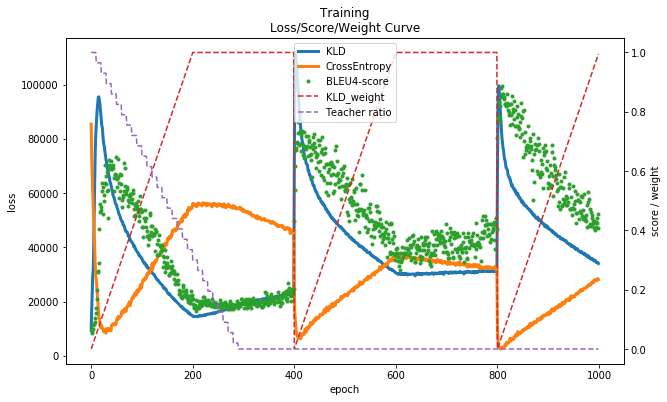
\includegraphics[width=\linewidth]{Images/curvesv3.png} 
\caption{Loss, Score, Weight Curves when training with lr=0.001}
\end{figure}

I find higher average score after each scope.

% --------------------------------------------------------------
%     You don't have to mess with anything below this line.
% --------------------------------------------------------------
 
\end{document}